%---------------------------------------------
%	PACKAGES AND OTHER DOCUMENT CONFIGURATIONS
%---------------------------------------------
\documentclass[
	letterpaper, % Letter Paper (Required for 4490Z)
	10pt, % Font Size %% MODIFY : FOR SUBMISSION ONLY - 10 NORMALLY
	%twoside, % Commented out for fixed headers/footers
]{journalArticle}

% BibLaTeX bibliography file
\addbibresource{references.bib}

% Running Header
\runninghead{Gavigan, Riley}

% Footer Content
\footertext{}

% Page Counter Starting Number
\setcounter{page}{1}

%---------------------------------------------
%	TITLE SECTION
%---------------------------------------------
\title{Explaining embedding results for scoring alignments}

% Authors are listed in a comma-separated list with superscript numbers indicating affiliations
\author{
	Riley Gavigan\\\normalsize{Thesis Supervisor: Lucian Ilie, Course Instructor: Nazim Madhavji}\\\footnotesize{Department of Computer Science, University of Western Ontario, London, N6A 5B7, Ontario, Canada}
}

% Affiliations are output in the \date{} command
\date{February 1, 2024\\}

% Full-width General Abstract
\renewcommand{\maketitlehookd}{%
	\begin{abstract}
		\noindent Abstract Content Here
	\end{abstract}
}
%------------------------------------------
\begin{document}

\maketitle % Output the title section
%---------------------------------------------
%	INTRODUCTION
%---------------------------------------------
\section{Introduction}
Proteins are one of the four molecules of life. Finding similarities among protein sequences is essential in identifying protein structure and function. This is done by computing alignments between sequences. The BLAST program\footnote{Exceeds 108,000 citations, according to Google Scholar.} is one of the most widely used tools in science \autocite{Atschul:1990}. An essential part of BLAST is the scoring function; the most widely used functions are provided by the BLOSUM matrices \autocite{Henikoff:1992}.

Sequence similarity is essential in sequence analysis for DNA, RNA, and peptide sequences \autocite{Ofer:2021}. Peptide sequence alignment is the most complex case, with a language of 20 common amino acids forming a theoretically countably infinite amount of unique peptide sequences shown in Equation \ref{eq:peptideinfinity} by taking the Cartesian product.

\begin{equation}
    {Theoretical\, Limit} = \prod_{k=1}^{\infty} |A| = \prod_{k=1}^{\infty} 20 = 20 \times 20 \times \ldots
    \label{eq:peptideinfinity}
\end{equation}

While there is theoretically a countably infinite number of peptide sequences, the observed sequences in living organisms are constrained by biological, genetic, and functional factors. For example, the average eukaryotic protein size is \(353 \pm 62.5\) residues \autocite{Nevers:2023}.

The \textit{E}-score protein alignment scoring method \autocite{Ashrafzadeh:2023} outperforms state-of-the-art methods, supported by comparing ProtT5 \autocite{Elnaggar:2021} \textit{E}-score results with BLOSUM45 \autocite{Henikoff:1992,Ashrafzadeh:2023}.

\textit{E}-score uses Transformer models to produce contextual embeddings for the residues in peptide sequences. Model information is available in Table \ref{tab:transformers}. These models are based off of their Natural Language Processing (NLP) equivalents \autocite{Raffel:2020, Devlin:2018, Zhenzhong:2020, Yang:2022, Rives:2021}.

Contextual embeddings are embeddings produced by the self-attention mechanism in the Transformer architecture \autocite{Vaswani:2017}, which is shown in Figure \ref{fig:transformer}. Similar to word embeddings in NLP, they describe the position of a residue in a high-dimensional vector space.

\begin{figure} % Single column figure
    \begin{center}
	   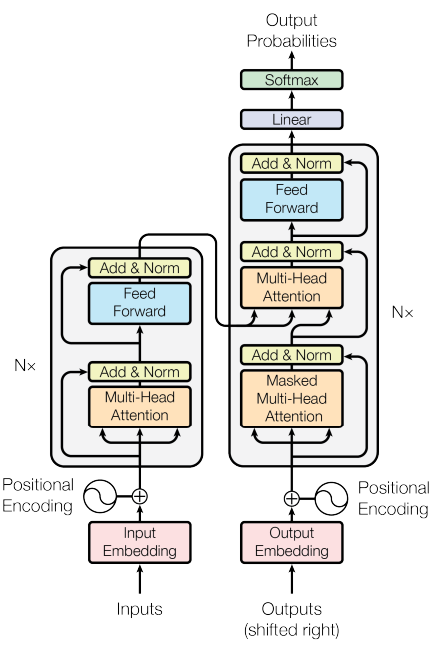
\includegraphics[width=0.6\linewidth]{Figures/transformer.png}
    \end{center}
	\caption{Transformer model architecture \autocite{Vaswani:2017}. Encoder is on the left; decoder is on the right.}
    \vspace{-5mm}
	\label{fig:transformer}
\end{figure}

\begin{table*} % Two column table
	\caption{Transformer models available in the \textit{E}-score method; \(n=\) number of residues. ProtT5, ProtBert, ProtAlbert, and ProtXLNet come from ProtTrans \autocite{Elnaggar:2021}. ESM1b and ESM2 come from the Meta Fundamental AI Research Protein Team \autocite{Rives:2021}.}
	\centering
	\begin{tabular}{ |c|c|c|c|c| }
		\toprule
		Model & Architecture & Embedding Dim & Pre-Trained Dataset & Training Method \\
		\midrule
		ProtT5 & Encoder-Decoder & n * 1024 & UniRef50 & Text-to-Text \\
        ESM1b & Encoder & n * 1280 & UniRef50 & Masked Language Modeling \\
        ESM2 & Encoder & n * 1280 & UniRef50 & Masked Language Modeling \\
		ProtBert & Encoder & n * 1024 & UniRef100 & Masked Language Modeling \\
		ProtAlbert & Encoder & n * 4096 & UniRef100 & Masked Language Modeling \\
        ProtXLNet & Decoder & n * 1024 & UniRef100 & Permutation Language Modeling \\
		\bottomrule
	\end{tabular}
	\label{tab:transformers}
\end{table*}

Contextual embeddings produced for protein sequences have many important applications in biology, including structure prediction \autocite{Senior:2020, Yang:2019, Jumper:2021} and function prediction \autocite{Kulmanov:2019, Gligorijevic:2021, Lai:2021}. 

The \textit{E}-score alignment method is another application for these embeddings, outperforming the state-of-the-art methods \autocite{Ashrafzadeh:2023} by completely changing the way alignments are computed.

The embedding vector produced for each protein residue varies based on the model that was used. For example, the embedding for a protein sequence of 310 residues using ProtT5 will have the dimensions [310, 1024]. The embedding dimensions are outlined in Table \ref{tab:transformers}. The dimensionality of the embedding vectors represents the number of features encoded in the embedding, and is a fixed value for a given model.

The embeddings produced by a model for a protein \(P\), calculated in Equation \ref{eq:embedding}, are used as the input to calculate the cosine similarity.

\begin{equation}
    E(P) = GetEmbeddings(Model = ProtT5)
    \label{eq:embedding}
\end{equation}

Calculating the cosine similarity between two vectors \(A = (A_i)_{i=1..n}\) and \(B = (B_i)_{i=1..n}\) is shown in Equation \ref{eq:cossim}.

\begin{equation}
    \begin{aligned}
        CosSim(A, B) = cos(\theta) \equiv \frac{A \cdot B}{\Vert A \Vert \Vert B \Vert} %\\ 
        \equiv \frac{\sum\limits_{i=1}^{n} A_iB_i}{\sqrt{\sum\limits_{i=1}^{n} A_i^2}\sqrt{\sum\limits_{i=1}^{n} B_i^2}}
    \end{aligned}
	\label{eq:cossim}
\end{equation}

\textit{E}-score is calculated by taking the cosine similarity between the embedding vector for two residues (\(i, j\)), shown in Equation \ref{eq:escore} where \(P_1\) and \(P_2\) are proteins \autocite{Ashrafzadeh:2023}.

\begin{equation}
    \textit{E}\mbox{-}score(i,j) = CosSim(E(P_1)_i, E(P_2)_j)
    \label{eq:escore}
\end{equation}

In calculating sequence alignment using the \textit{E}-score method, the cosine similarity results were mostly  mostly less than \(\frac{\pi}{2}\). It was also determined that ProtT5 performed better than the other models \autocite{Ashrafzadeh:2023}.

In this paper, I explain significant qualitative and quantitative differences and similarities between the models in Table \ref{tab:transformers}. Combined with visualization and analysis of embedding vector and cosine similarity distributions, I propose the contributing factors to better \textit{E}-score performance.

Inference is applied to describe the procedure and techniques for fine-tuning ProtT5 and other models to produce better embeddings for alignment.

%---------------------------------------------
%	MATERIALS AND METHODS
%---------------------------------------------
\section{Materials and Methods}

\subsection{Transformers}
T5 is an encoder-decoder model; it uses both the encoder and decoder of the Transformer architecture. Explain how this excels and how it relates to E-Score and why T5 performs best. Mention the dimension of embeddings. Mention the training procedure.

BERT and ALBERT are auto-encoder models; they only use the encoder of the Transformer architecture. Explain how this excels and how it relates to their performance. Mention the dimension of embeddings. Mention the training procedure.

XLNet is an auto-regressive model; it only uses the decoder of the Transformer architecture. Explain how this excels and how it relates to their performance. Mention the dimension of embeddings. Mention the training procedure.

ESM1b and ESM2 are also auto-encoder models; they only use the encoder of the Transformer architecture and are based on RoBERTa. Mention the dimension of embeddings. Mention the training procedure.

Compare BERT, ALBERT, ESM1b and ESM2 because they are all auto-encoding models. Their differences and similarities, and their E-score results observed.

\subsection{Embedding vectors}

\subsubsection{Data}
Embedding vectors will be analyzed between the available models on this representative data.

\subsubsection{Normalizing vector results}

\subsubsection{Visualizing normalized results}

\subsubsection{Analyzing visualizations and data}

\subsection{Cosine similarity}

\subsubsection{Data}
Cosine similarity will be analyzed between embedding vectors between different models on this representative data.

\subsubsection{Visualizing cosine similarity}

\subsubsection{Analyzing visualizations and data}

\subsection{Fine-tuning ProtT5}

\subsubsection{Data}
ProtT5 will be fine-tuned with representative data from...

\subsubsection{PEFT and LoRA}

\subsubsection{Compute Power}

\subsubsection{Intuition and reasoning}



%---------------------------------------------
%	RESULTS
%---------------------------------------------
\section{Results}

\subsection{Embedding distributions}

\subsection{Cosine similarity}

\subsection{Model performance}

\subsection{Fine-tuning}

%---------------------------------------------
%	DISCUSSION AND CONCLUSION
%---------------------------------------------
\section{Discussion and Conclusion}


%---------------------------------------------
%	ACKNOWLEDGEMENTS
%---------------------------------------------
\section{Acknowledgements}
Dr. Lucian Ilie provided thesis supervision and guidance. This research built upon the initial \textit{E}-score method research \autocite{Ashrafzadeh:2023}.

%---------------------------------------------
%	Supplementary data
%---------------------------------------------
\section{Supplementary information}
The proposal for this research was completed and approved November 2023, and can be found online\footnote{https://www.rileygavigan.com/e-score-proposal.pdf}.

A supplementary file containing Supplementary Tables 1-N is available online\footnote{https://www.rileygavigan.com/e-score-data.pdf}.

%---------------------------------------------
%	REFERENCES
%---------------------------------------------
\printbibliography % Output the bibliography
%---------------------------------------------
\end{document}